%%%%%%%%%%%%%%%%%%%%%%%%%%%%%%%%%%%%%%%%%%%%%%%%%%%%%%%%%%%%%%%%%%
\section{방법론}\label{sec:methodology}
%%%%%%%%%%%%%%%%%%%%%%%%%%%%%%%%%%%%%%%%%%%%%%%%%%%%%%%%%%%%%%%%%%

\subsection{2단계 직접 배치법}\label{subsec:direct_collocation}

식~\eqref{eq:ocp}에서 정의한 연속 최적 제어 문제를 2단계 직접 배치법(two-pass direct collocation)을 통해 유한 차원의 비선형 프로그래밍(NLP) 문제로 변환한다. 이 혼합 방법은 에르미트-심프슨 배치법의 균일 샘플링 장점과 르장드르-가우스-로바토(LGL) 유사 스펙트럴 방법의 높은 정확도를 결합한 것이다 \citep{Hargraves1987,Rao2025,Fahroo2002}.

2단계 접근법의 동기는 유사 스펙트럴 방법의 근본적 한계에서 비롯된다. LGL 노드는 정의역 경계 근처에 밀집되어, 최적 해의 추력 집중 영역(피크)과 일치하지 않을 수 있다. 피크 위치를 \textit{사전에(a priori)} 알 수 없으므로, 먼저 균일 분포 노드로 예비 최적화를 수행하여 추력 프로파일 구조를 파악한 후, 적응적 노드 배치로 정밀 최적화를 수행한다.

\subsubsection{1단계: 에르미트-심프슨 배치법}

1단계에서는 균일 간격 노드를 사용하는 에르미트-심프슨 배치법을 적용하여 예비 해를 구하고 추력 피크 위치를 식별한다. 전이 기간 $[0, T_f]$를 폭 $h = T_f/M$인 $M$개의 동일 구간으로 분할한다. 각 구간 $[t_k, t_{k+1}]$ 내에서 상태 궤적을 3차 에르미트 다항식으로 근사하고, 심프슨 규칙을 사용하여 구간 중점에서 배치를 적용한다.

각 구간에 대한 배치 구속조건은 다음과 같다:
\begin{align}
\mathbf{x}_{k+1} &= \mathbf{x}_k + \frac{h}{6}\left[\mathbf{f}_k + 4\mathbf{f}_{k+\frac{1}{2}} + \mathbf{f}_{k+1}\right] \label{eq:simpson_continuity} \\
\mathbf{x}_{k+\frac{1}{2}} &= \frac{1}{2}(\mathbf{x}_k + \mathbf{x}_{k+1}) + \frac{h}{8}(\mathbf{f}_k - \mathbf{f}_{k+1}) \label{eq:hermite_midpoint}
\end{align}
여기서 $\mathbf{f}_k = \mathbf{f}(\mathbf{x}_k, \mathbf{u}_k)$는 노드 $k$에서 평가한 동역학을 나타낸다. 비용 함수는 심프슨 구적법으로 근사한다:
\begin{equation}
J \approx \sum_{k=0}^{M-1} \frac{h}{6}\left[\|\mathbf{u}_k\|^2 + 4\|\mathbf{u}_{k+\frac{1}{2}}\|^2 + \|\mathbf{u}_{k+1}\|^2\right]
\end{equation}

데이터베이스 구축에는 $M = 30$ 구간을 사용하여, 61개의 배치점(31개 주 노드와 30개 중점)과 약 550개의 결정 변수를 생성한다. 균일 노드 분포는 추력 피크의 시간적 위치에 관계없이 피크를 포착할 수 있도록 한다.

\subsubsection{피크 탐지}

1단계 수렴 후, 추력 크기 프로파일 $\|\mathbf{u}(t)\|$를 분석하여 추력 집중 영역에 해당하는 극대값을 식별한다. Section~\ref{subsec:classification}에서 기술하는 돌출도 기반 알고리즘으로 피크를 탐지하며, 인접 피크 간 최소 간격은 $T_f/10$으로 설정한다. 탐지된 피크 수에 따라 추력 프로파일 분류(단봉형, 쌍봉형, 다봉형)가 결정되며, 2단계의 페이즈 구조를 결정하는 데 활용된다.

\subsubsection{2단계: 다중 페이즈 LGL 배치법}

2단계에서는 탐지된 피크 구조에 기반하여 전이 구간을 별도의 페이즈로 분할하는 다중 페이즈 정식화를 적용한다. 각 페이즈는 LGL 노드로 독립적으로 이산화되며, 피크 영역에는 높은 노드 밀도를, 관성 비행 영역에는 낮은 노드 밀도를 배정한다.

$n_p$개의 피크가 탐지된 문제의 경우, 전이 구간을 $2n_p - 1$개의 페이즈로 분할한다: 탐지된 피크 시간을 중심으로 $n_p$개의 피크 페이즈와 그 사이에 $n_p - 1$개의 관성 비행 페이즈를 배치한다. 페이즈 경계는 최적화 변수로 포함되어, 솔버가 피크 위치를 정밀하게 조정할 수 있도록 한다.

$[T_{p-1}, T_p]$ 구간을 포괄하는 각 페이즈 $p$ 내에서 시간 좌표를 $\sigma \in [-1, 1]$로 변환한다:
\begin{equation}
t = T_{p-1} + \frac{T_p - T_{p-1}}{2}(\sigma + 1)
\end{equation}

페이즈 $p$ 내의 상태와 제어는 $N_p + 1$개의 LGL 노드에서 근사한다. 상태 궤적은 라그랑주 보간 다항식으로 표현한다:
\begin{equation}
\mathbf{x}^{(p)}(\sigma) \approx \sum_{j=0}^{N_p} \mathbf{x}_j^{(p)} L_j(\sigma)
\end{equation}
동역학 구속조건은 다음과 같이 적용한다:
\begin{equation}
\frac{2}{T_p - T_{p-1}} \sum_{j=0}^{N_p} D_{ij}^{(p)} \mathbf{x}_j^{(p)} = \mathbf{f}(\mathbf{x}_i^{(p)}, \mathbf{u}_i^{(p)})
\end{equation}
여기서 $\mathbf{D}^{(p)}$는 페이즈 $p$의 LGL 미분 행렬이다.

페이즈 경계에서의 연속성은 연결 구속조건을 통해 보장한다:
\begin{equation}
\mathbf{x}^{(p)}(\sigma = 1) = \mathbf{x}^{(p+1)}(\sigma = -1), \quad p = 1, \ldots, P-1
\end{equation}

비용 함수는 전체 페이즈의 기여를 합산한다:
\begin{equation}
J \approx \sum_{p=1}^{P} \frac{T_p - T_{p-1}}{2} \sum_{j=0}^{N_p} w_j^{(p)} \|\mathbf{u}_j^{(p)}\|^2
\end{equation}
여기서 $w_j^{(p)}$는 페이즈 $p$의 LGL 구적 가중치이다.

데이터베이스 구축에서 피크 페이즈는 $N_{\text{peak}} = 15$개 노드로, 관성 비행 페이즈는 $N_{\text{coast}} = 8$개 노드로 이산화한다. 1단계의 해를 LGL 노드에 보간하여 초기 추정치(warm-start)로 제공함으로써 수렴 신뢰도를 크게 향상시킨다.

\subsubsection{구현}

두 최적화 단계 모두 CasADi 기호 연산 프레임워크 \citep{Andersson2019}의 Opti 스택 인터페이스로 정식화하고, 내부점 솔버 IPOPT \citep{Waechter2006}와 MUMPS 선형 솔버로 풀이한다. CasADi는 비용 함수와 구속조건의 자동 미분을 제공하여, 수동 유도 없이 정확한 야코비안과 헤시안을 IPOPT에 공급한다. 1단계에서는 완화된 수렴 허용오차($10^{-4}$)를 사용하여 빠른 예비 해를 구하고, 2단계에서는 엄격한 허용오차($10^{-6}$)를 적용하여 최종 고정밀 해를 산출한다. 1단계의 해를 LGL 노드에 보간하여 2단계의 초기 추정치로 활용한다.

2단계 접근법은 일반적으로 최신 워크스테이션에서 사례당 3초 미만이 소요되어, 대규모 궤적 데이터베이스의 체계적 생성을 가능하게 한다.

\subsection{구성 공간 및 샘플링}\label{subsec:configuration}

궤도전이 기하가 최적 추력 프로파일 특성에 미치는 영향을 체계적으로 조사하기 위해, 정밀하게 정의된 구성 공간에 대한 매개변수 연구를 수행한다. 구성 매개변수, 범위, 샘플링 전략을 아래에 기술한다.

\subsubsection{구성 매개변수}

구성 공간은 궤도전이 기하를 특성화하는 다섯 가지 주요 매개변수로 정의한다:

\begin{itemize}
\item \textit{장반경 변화량} ($\Delta a = a_f - a_0$): 도착 궤도와 출발 궤도 간 장반경 차이이다. 이 매개변수는 전이의 에너지 요구량을 지배하며, 궤도 상승(예: 재진입 후 고도 회복) 및 궤도 강하(예: 제어 탈궤도) 시나리오를 모두 포괄하여, 재사용 우주비행체(ReUSV) 임무에 적합하다.

\item \textit{경사각 변화량} ($\Delta i = i_f - i_0$): 궤도면 경사각의 변화량이다. 궤도면 변경은 궤도역학에서 가장 비용이 큰 기동 중 하나로, 궤도면에 수직한 속도 변화가 필요하다.

\item \textit{출발 이심률} ($e_0$): 출발 궤도의 이심률이다. $e_0$를 독립 매개변수로 포함함으로써 타원 주차 궤도에서 출발하는 전이를 수용하며, 이는 ReUSV 임무에서 대기 스킵 또는 공기제동 기동 후 자연스럽게 발생한다.

\item \textit{도착 이심률} ($e_f$): 목표 궤도의 이심률이다. $e_f$를 $e_0$와 독립적으로 취급하면 원형화 기동($e_0 > 0, e_f = 0$) 및 타원 목표 궤도로의 전이를 모두 연구할 수 있다.

\item \textit{전이시간 범위} ($[T_{\min}, T_{\max}]$): 자유 전이시간 $T_f$의 허용 범위로, 초기 궤도주기 $T_0 = 2\pi\sqrt{a_0^3/\mu}$ 단위로 표현한다. 본 연구는 $T_f/T_0 \leq 1.2$인 단기간 전이에 집중하며, 이는 고추력형 연속 추력 운용의 특성인 1회전 미만 기동에 해당한다.
\end{itemize}

또한, 초기 궤도 고도($h_0 = a_0 - R_E$)는 슬라이스별 분석을 위한 보조 매개변수로 활용하여, 궤도 고도에 따른 분류 경계의 변화를 조사한다.

승교점 적경은 일정하게 유지한다($\Omega_0 = \Omega_f = 0$). $J_2$ 대역조화 함수를 포함한 2체 중력장---지구 극축에 대한 회전 대칭이 보존됨---하에서 $\Omega$의 절대값은 궤적 최적화에 영향을 미치지 않으므로, 이 축약은 일반성의 손실 없이 유효하다 \citep{Vallado2013}. 근지점 편각도 일정하게 유지한다($\omega_0 = \omega_f = 0$). 원궤도($e = 0$)의 경우 $\omega$는 정의되지 않으므로 이 선택은 자명하게 유효하다. 타원 궤도($e > 0$)의 경우 $\omega$를 고정하면 근점선 방향이 제한되며, 독립 매개변수로서의 $\omega$의 영향은 향후 연구로 남긴다 \citep{Curtis2020}.

\subsubsection{매개변수 범위}

매개변수 범위는 운용상 의미 있는 LEO 전이 시나리오를 포괄하도록 선정한다:

\begin{table}[ht]
\centering
\caption{매개변수 연구를 위한 구성 매개변수 범위.}
\label{tab:param_ranges}
\begin{tabular}{lccc}
\hline
매개변수 & 기호 & 범위 & 단위 \\
\hline
장반경 변화량 & $\Delta a$ & [TBD] & km \\
경사각 변화량 & $\Delta i$ & [TBD] & deg \\
출발 이심률 & $e_0$ & $[0,\;\text{TBD}]$ & -- \\
도착 이심률 & $e_f$ & $[0,\;\text{TBD}]$ & -- \\
전이시간 범위 & $T_f/T_0$ & $[\text{TBD},\; 1.2]$ & -- \\
초기 고도 & $h_0$ & $\{400, 600, 800, 1000\}$ & km \\
\hline
\end{tabular}
\end{table}

장반경 범위는 궤도 강하 기동(음의 $\Delta a$, ReUSV 제어 탈궤도 또는 충돌 회피에 활용)과 궤도 상승 기동(양의 $\Delta a$, 재진입 후 궤도 회복 또는 위성군 배치에 활용)을 모두 포함한다. 경사각 변화 범위는 지상궤적 최적화 및 임무 위상 조정을 위한 실용적 궤도면 변경 요구를 포괄한다. 이심률 매개변수 $e_0$와 $e_f$는 독립적으로 취급하여, 원형-원형($e_0 = e_f = 0$), 타원-원형(원형화), 원형-타원, 타원-타원 전이 등 다양한 전이 기하의 연구를 가능하게 한다. 전이시간 상한 $T_f/T_0 \leq 1.2$는 데이터베이스를 1회전 미만 전이로 제한하며, 이는 신속한 궤도 조정이 요구되는 ReUSV 궤도 회복 및 랑데부 시나리오에 적합한 단기간 기동의 특성에 해당한다.

\subsubsection{적응적 샘플링 전략}

분류 경계를 적절히 해상하기 위해 과도한 샘플이 필요한 균일 격자 샘플링 대신, 적응적 샘플링 전략을 채택한다. 이 접근법은 두 단계로 구성된다:

\textit{1단계: 초기 커버리지 샘플링.} 라틴 하이퍼큐브 샘플링(LHS)을 사용하여 5차원 매개변수 공간 $(\Delta a, \Delta i, e_0, e_f, T_{\max}/T_0)$ 전체에 분포된 초기 샘플 $N_{\text{init}}$개를 생성한다. 이 공간 충진 설계는 군집화를 방지하면서 구성 공간의 적절한 커버리지를 보장한다.

\textit{2단계: 경계 집중 적응적 샘플링.} 초기 샘플에 대해 가우시안 프로세스(GP) 분류기를 훈련하여, 매개변수 공간 전체에서 추력 프로파일 클래스 소속의 확률적 예측을 제공한다. 분류 불확실성이 가장 높은 위치에서 새로운 샘플을 반복적으로 선정하여, 서로 다른 추력 프로파일 영역 간 경계 부근에 샘플링 노력을 집중한다. 이 접근법은 능동 학습 원리에 기반하며 \citep{Settles2009}, 동역학 시스템의 분류 경계 식별에 성공적으로 적용된 바 있다 \citep{Lee2023}. 엔트로피 기반 획득 함수는 정보이론적 해석을 허용한다: 고엔트로피 위치에서의 샘플링은 분류 경계에 대한 불확실성을 최대로 감소시켜, 매개변수 공간 체적이 아닌 경계 복잡도에 비례하는 거의 최적의 샘플 복잡도를 달성한다. GP 기반 샘플링 절차의 수학적 세부사항은 부록~\ref{app:gp_sampling}에 제시한다.

적응적 샘플링은 최대 $N_{\text{max}}$개 샘플에 도달하거나 최대 분류 불확실성이 수렴 임계값 이하로 감소할 때까지 계속된다. [TBD: 샘플 수 및 수렴 통계는 데이터베이스 재생성 후 갱신 예정.]

\subsection{추력 프로파일 분류}\label{subsec:classification}

최적 추력 프로파일의 분류는 2단계 최적화(Section~\ref{subsec:direct_collocation})의 1단계에서 수렴된 해에서 식별된 추력 크기 피크의 수와 특성에 기반한다.

\subsubsection{분류 기준}

피크 수에 따라 세 가지 분류를 정의한다:

\begin{itemize}
\item \textit{단봉형} (Class 0): 단일 추력 피크. 추력 크기 프로파일이 하나의 지배적 극대값을 나타내며, 단일 궤도 위치에서의 집중적 추진 노력에 해당한다. 이 패턴은 단일 임펄스 기동에 대응한다.

\item \textit{쌍봉형} (Class 1): 두 개의 추력 피크. 프로파일이 저추력 또는 관성 비행 영역으로 분리된 두 개의 뚜렷한 극대값을 보인다. 이 패턴은 호만 전이와 같은 고전적 2-임펄스 기동에 대응한다.

\item \textit{다봉형} (Class 2): 세 개 이상의 추력 피크. 프로파일이 다수의 뚜렷한 극대값을 나타내며, 이중타원 전이와 같은 다중 임펄스 전략에 대응한다.
\end{itemize}

\subsubsection{피크 탐지 알고리즘}

피크는 합성 추력 크기 프로파일 $\|\mathbf{u}(t)\|$에 적용한 돌출도 기반 탐지 알고리즘으로 식별한다(Fig.~\ref{fig:peak_detection_schematic}). 극대값이 유의미한 피크로 분류되려면, 돌출도---인접한 두 극소값 중 높은 값으로부터의 높이---가 전역 최대 추력 크기의 10\%를 초과해야 한다. 이 기준은 미세한 변동을 걸러내면서도 물리적으로 의미 있는 추력 집중 영역을 보존한다. 또한, 인접 피크는 시간상 최소 $T_f/10$ 이상 분리되어야 하며, 이는 배치 해의 수치 진동으로 인한 허위 피크 탐지를 방지한다. 이 두 임계값은 전이 구성의 전 범위에서 강건한 분류를 제공하면서도 최적화 해의 미세한 변동에 둔감하도록 경험적으로 결정하였다.

\begin{figure}[ht]
\centering
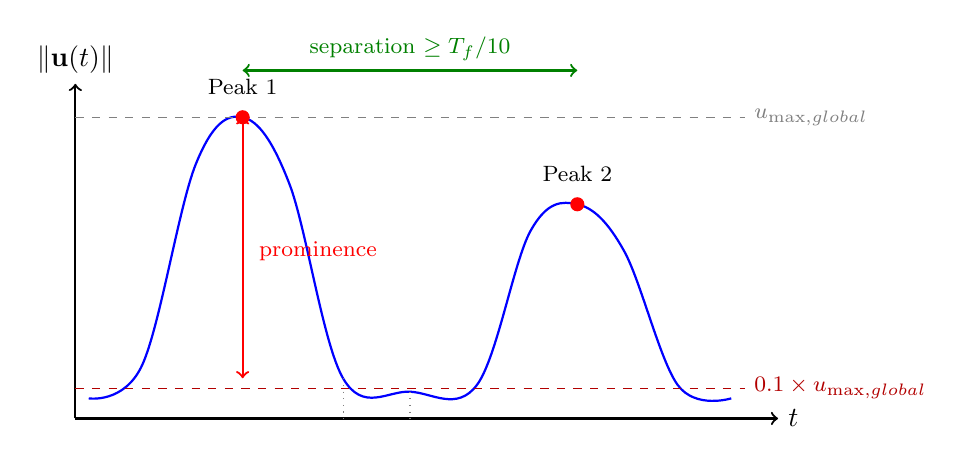
\begin{tikzpicture}[scale=0.85]
  % Axes
  \draw[->,thick] (0,0) -- (10.5,0) node[right] {$t$};
  \draw[->,thick] (0,0) -- (0,5.0) node[above] {$\|\mathbf{u}(t)\|$};
  % Thrust profile (synthetic bimodal)
  \draw[thick,blue] plot[smooth,tension=0.6] coordinates {
    (0.2,0.3) (1.0,0.8) (1.8,3.8) (2.5,4.5) (3.2,3.5) (4.0,0.6)
    (5.0,0.4) (6.0,0.5) (6.8,2.8) (7.5,3.2) (8.2,2.5) (9.0,0.5) (9.8,0.3)
  };
  % Global max dashed line
  \draw[dashed,gray] (0,4.5) -- (10,4.5);
  \node[gray,right] at (10,4.5) {\footnotesize $u_{\max,\text{global}}$};
  % 10% threshold line
  \draw[dashed,red!70!black] (0,0.45) -- (10,0.45);
  \node[red!70!black,right] at (10,0.45) {\footnotesize $0.1\times u_{\max,\text{global}}$};
  % Prominence arrow (peak 1)
  \draw[<->,thick,red] (2.5,0.6) -- (2.5,4.5);
  \node[red,right] at (2.6,2.5) {\footnotesize prominence};
  % Local minimum between peaks
  \draw[dotted,gray] (4.0,0.6) -- (4.0,0);
  \draw[dotted,gray] (5.0,0.4) -- (5.0,0);
  % Separation arrow
  \draw[<->,thick,green!50!black] (2.5,5.2) -- (7.5,5.2);
  \node[green!50!black,above] at (5.0,5.2) {\footnotesize separation $\geq T_f/10$};
  % Peak markers
  \fill[red] (2.5,4.5) circle (3pt);
  \fill[red] (7.5,3.2) circle (3pt);
  \node[above] at (2.5,4.7) {\footnotesize Peak 1};
  \node[above] at (7.5,3.4) {\footnotesize Peak 2};
\end{tikzpicture}
\caption{돌출도 기반 피크 탐지 기준의 도식. 수직 화살표는 Peak~1의 돌출도(인접 극소값으로부터의 높이)를, 수평 화살표는 인접 피크 간 요구되는 최소 시간 분리를 나타낸다.}
\label{fig:peak_detection_schematic}
\end{figure}


%%%%%%%%%%%%%%%%%%%%%%%%%%%%%%%%%%%%%%%%%%%%%%%%%%%%%%%%%%%%%%%%%%
\section{결과: 추력 프로파일 데이터베이스}\label{sec:results_database}
%%%%%%%%%%%%%%%%%%%%%%%%%%%%%%%%%%%%%%%%%%%%%%%%%%%%%%%%%%%%%%%%%%

\subsection{데이터베이스 개요}\label{subsec:database_overview}

Section~\ref{subsec:configuration}에서 기술한 적응적 샘플링 전략을 네 개의 초기 고도 슬라이스($h_0 = 400$, 600, 800, 1000~km)에 독립적으로 적용하였다. Table~\ref{tab:db_summary}에 구축된 궤적 데이터베이스를 요약한다.

\begin{table}[ht]
\centering
\caption{궤적 데이터베이스 요약. [TBD: 확장된 5차원 구성 공간으로 데이터베이스 재생성 후 값 갱신 예정.]}
\label{tab:db_summary}
\begin{tabular}{rrrrccc}
\hline
$h_0$ [km] & 전체 & 수렴 & 비율 & 단봉형 & 쌍봉형 & 다봉형 \\
\hline
400 & [TBD] & [TBD] & [TBD] & [TBD] & [TBD] & [TBD] \\
600 & [TBD] & [TBD] & [TBD] & [TBD] & [TBD] & [TBD] \\
800 & [TBD] & [TBD] & [TBD] & [TBD] & [TBD] & [TBD] \\
1000 & [TBD] & [TBD] & [TBD] & [TBD] & [TBD] & [TBD] \\
\hline
합계 & [TBD] & [TBD] & [TBD] & [TBD] & [TBD] & [TBD] \\
\hline
\end{tabular}
\end{table}

[TBD: 수렴률 및 통계.] 미수렴 사례는 요구되는 궤도요소 변화가 가용 전이시간에 비해 큰 매개변수 공간의 경계 부근에서 집중적으로 발생할 것으로 예상된다. 물리적 추력 상한 $u_{\max}$ 초과로 미수렴을 귀인하던 이전 정식화와 달리, $T_f$를 자유 변수로 두고 완화된 수치 안전장치 $u_{\max}$를 적용하는 현재 정식화에서는 미수렴이 주로 규정된 전이시간 범위 $[T_{\min}, T_{\max}]$가 요구 궤도 변화를 달성하기에 불충분한 경우에 기인한다.

적응적 샘플링은 분류 경계 부근에 샘플을 효과적으로 집중시켰다(Fig.~\ref{fig:sampling_progress}). [TBD: 엔트로피 수렴 통계는 데이터베이스 재생성 후 갱신 예정.]

\begin{figure}[ht]
\centering
\includegraphics[width=\columnwidth]{figures/fig7_sampling_progress.pdf}
\caption{각 초기 고도 슬라이스에 대한 적응적 샘플링 수렴 과정으로, 누적 평가 샘플 수를 나타낸다.}
\label{fig:sampling_progress}
\end{figure}

\subsection{추력 프로파일 유형 분포}\label{subsec:type_distribution}

세 가지 추력 프로파일 유형---단봉형, 쌍봉형, 다봉형---을 데이터베이스에서 선정한 대표 사례를 통해 Fig.~\ref{fig:representative_profiles}에 예시한다.

\begin{figure*}[t]
\centering
\includegraphics[width=\textwidth]{figures/fig1_representative_profiles.pdf}
\caption{각 분류 유형의 대표 추력 크기 프로파일: (a)~단일 추력 피크를 가진 단봉형, (b)~관성 비행 영역으로 분리된 두 개의 뚜렷한 추력 피크를 가진 쌍봉형, (c)~세 개 이상의 피크를 가진 다봉형. [갱신 예정: 갱신된 데이터베이스에서 정확히 1, 2, 3개 피크를 가진 명확한 예시 선정.]}
\label{fig:representative_profiles}
\end{figure*}

단봉형 프로파일(Fig.~\ref{fig:representative_profiles}a)은 단일의 매끄러운 추력 피크를 나타내며, 하나의 궤도 위치에서 추진 노력을 집중한다. 이 패턴은 짧은 전이시간에서 우세하며, 우주선이 다중 추력 아크를 형성할 충분한 시간이 없는 경우에 해당한다.

쌍봉형 프로파일(Fig.~\ref{fig:representative_profiles}b)은 거의 0에 가까운 추력의 관성 비행 영역으로 분리된 두 개의 뚜렷한 추력 피크를 보인다. 이 구조는 출발 및 도착 궤도 위치에서 추력이 집중되는 고전적 2-임펄스 호만 전이 기하에 직접 대응한다. [TBD: 쌍봉형 사례 비율 갱신 예정.]

다봉형 프로파일(Fig.~\ref{fig:representative_profiles}c)은 관성 비행 아크가 사이에 개재된 세 개 이상의 추력 피크를 나타낸다. 현재 데이터베이스가 1회전 미만 전이($T_f/T_0 \leq 1.2$)로 제한되어 있으므로, 다봉형 프로파일은 다중 공전 영역에 비해 낮은 빈도로 발생할 것으로 예상되며, 주로 큰 고도-경사각-이심률 복합 변화에서 단일 궤도 공전 내에서도 다중 연소 전략이 에너지적으로 유리한 경우에 나타난다.

\begin{figure*}[t]
\centering
\includegraphics[width=\textwidth]{figures/fig2_representative_trajectories.pdf}
\caption{Fig.~\ref{fig:representative_profiles}의 대표 프로파일에 대응하는 3차원 ECI 궤적: (a)~단봉형, (b)~쌍봉형, (c)~다봉형. [갱신 예정: 점 밀도 증가, 궤적선 두께 증가, 가속도 비례 색상 매핑.]}
\label{fig:representative_trajectories}
\end{figure*}

대응하는 3차원 궤적을 Fig.~\ref{fig:representative_trajectories}에 나타낸다. 단봉형 사례(a)는 거의 직접적인 전이 아크를 보이며, 쌍봉형 사례(b)는 타원형 호만 궤도를 닮은 전이 기하를 나타낸다. 다봉형 사례(c)는 기하학적으로 유리한 궤도 위치에서 다수의 뚜렷한 추력 아크를 가진 1회전 미만 궤적을 보인다.

Table~\ref{tab:class_cost}에 각 프로파일 클래스별 $L^2$ 비용 통계를 요약한다. 비용 $J$의 단위는 km$^2$/s$^3$(가속도 제곱의 시간 적분)이다. 차원적으로, 특성 속도 변화 $\Delta v$를 전이시간 $T_f$ 동안 수행하는 전이의 경우, 비용은 $J \sim (\Delta v)^2 / T_f$로 스케일되어, 기동 크기와 가용 전이시간 간의 절충을 반영한다.

\begin{table}[ht]
\centering
\caption{프로파일 클래스별 $L^2$ 비용 통계(수렴 사례만 포함). 비용 $J$의 단위는 km$^2$/s$^3$이다. [TBD: 데이터베이스 재생성 후 값 갱신 예정.]}
\label{tab:class_cost}
\begin{tabular}{lrcccc}
\hline
클래스 & 수량 & 평균 $J$ & 표준편차 $J$ & 최솟값 $J$ & 최댓값 $J$ \\
 & & [km$^2$/s$^3$] & [km$^2$/s$^3$] & [km$^2$/s$^3$] & [km$^2$/s$^3$] \\
\hline
단봉형 & [TBD] & [TBD] & [TBD] & [TBD] & [TBD] \\
쌍봉형 & [TBD] & [TBD] & [TBD] & [TBD] & [TBD] \\
다봉형 & [TBD] & [TBD] & [TBD] & [TBD] & [TBD] \\
\hline
\end{tabular}
\end{table}

\subsection{지배 인자 분석}\label{subsec:dominant_factors}

추력 프로파일 분류에 가장 강하게 영향을 미치는 구성 매개변수를 식별하기 위해, 분류 맵과 GP 분류기의 ARD 커널 길이척도를 분석한다.

\subsubsection{분류 맵}

Fig.~\ref{fig:classification_da_di}--\ref{fig:classification_di_T}에 각 고도 슬라이스에 대한 분류 경계의 2차원 투영을 나타낸다. 구성 공간이 5차원 $(\Delta a, \Delta i, e_0, e_f, T_f/T_0)$이므로, 각 2차원 맵은 나머지 세 매개변수를 대표값으로 고정하여 생성한다. [TBD: 각 투영에 대한 고정값 명시.] 이 맵들은 매개변수 공간에서 각 프로파일 유형과 관련된 영역을 보여준다.

\begin{figure*}[t]
\centering
\includegraphics[width=\textwidth]{figures/fig3_classification_da_di.pdf}
\caption{각 초기 고도에 대한 $\Delta a$--$\Delta i$ 평면의 분류 맵: (a)~$h_0 = 400$~km, (b)~$h_0 = 600$~km, (c)~$h_0 = 800$~km, (d)~$h_0 = 1000$~km.}
\label{fig:classification_da_di}
\end{figure*}

\begin{figure*}[t]
\centering
\includegraphics[width=\textwidth]{figures/fig4_classification_da_T.pdf}
\caption{각 초기 고도에 대한 $\Delta a$--$T_f/T_0$ 평면의 분류 맵.}
\label{fig:classification_da_T}
\end{figure*}

\begin{figure*}[t]
\centering
\includegraphics[width=\textwidth]{figures/fig5_classification_di_T.pdf}
\caption{각 초기 고도에 대한 $\Delta i$--$T_f/T_0$ 평면의 분류 맵.}
\label{fig:classification_di_T}
\end{figure*}

$\Delta a$--$T_f/T_0$ (Fig.~\ref{fig:classification_da_T}) 및 $\Delta i$--$T_f/T_0$ (Fig.~\ref{fig:classification_di_T}) 투영은 프로파일 유형 간 가장 명확한 분리를 나타내며, 전이시간 $T_f/T_0$가 추력 프로파일 형태를 결정하는 지배적 인자임을 시사한다. 반면, $\Delta a$--$\Delta i$ 투영(Fig.~\ref{fig:classification_da_di})은 클래스 간 더 많은 중첩을 보여, 궤도요소 변화만으로는 프로파일 유형을 예측하기에 불충분함을 시사한다. [TBD: $e_0$ 및 $e_f$를 포함한 투영 추가.]

분류 맵의 3차원 시각화(Fig.~\ref{fig:classification_3d})는 분류 경계가 매개변수 공간에서 곡면을 형성하며, $T_f/T_0$가 분리의 주축을 제공함을 확인한다.

\begin{figure}[ht]
\centering
\includegraphics[width=\columnwidth]{figures/fig6_classification_3d.pdf}
\caption{$h_0 = 800$~km에 대한 3차원 분류 맵.}
\label{fig:classification_3d}
\end{figure}

\subsubsection{ARD 길이척도 분석}

GP 분류기의 ARD 커널 길이척도는 분류가 각 입력 매개변수에 얼마나 민감하게 의존하는지를 정량화한다. 길이척도가 짧을수록 해당 차원을 따라 분류 함수가 더 빠르게 변하며, 이는 결과에 대한 더 강한 영향을 의미한다.

Table~\ref{tab:ard_lengthscales}에 각 고도 슬라이스별 ARD 길이척도를 제시한다. 확장된 5차원 구성 공간에서 $\ell_{e_0}$와 $\ell_{e_f}$ 두 개의 길이척도가 추가로 보고된다.

\begin{table}[ht]
\centering
\caption{초기 고도별 ARD 길이척도. 작은 값은 분류에 대한 더 강한 영향을 나타낸다. [TBD: 데이터베이스 재생성 후 값 갱신 예정.]}
\label{tab:ard_lengthscales}
\begin{tabular}{rccccc}
\hline
$h_0$ [km] & $\ell_{T_f/T_0}$ & $\ell_{\Delta a}$ & $\ell_{\Delta i}$ & $\ell_{e_0}$ & $\ell_{e_f}$ \\
\hline
400 & [TBD] & [TBD] & [TBD] & [TBD] & [TBD] \\
600 & [TBD] & [TBD] & [TBD] & [TBD] & [TBD] \\
800 & [TBD] & [TBD] & [TBD] & [TBD] & [TBD] \\
1000 & [TBD] & [TBD] & [TBD] & [TBD] & [TBD] \\
\hline
\end{tabular}
\end{table}

\begin{figure}[ht]
\centering
\includegraphics[width=\columnwidth]{figures/fig8_ard_lengthscales.pdf}
\caption{고도 슬라이스 간 ARD 길이척도 비교. [갱신 예정: 넓은 동적 범위를 수용하기 위해 종축에 대수 스케일 사용, 또는 Table~\ref{tab:ard_lengthscales}와 중복될 경우 제거 검토.]}
\label{fig:ard_lengthscales}
\end{figure}

[TBD: ARD 길이척도 분석은 5차원 결과로 갱신 예정.] 무차원 전이시간 $T_f/T_0$가 지배적 인자로 유지될 것으로 예상된다. $\Delta a$ 및 $\Delta i$와 비교한 이심률 매개변수 $e_0$ 및 $e_f$의 상대적 중요도를 통해, 1회전 미만 전이에서 궤도 형상이 추력 프로파일 형태 결정에 유의미한 역할을 하는지 밝힐 수 있을 것이다.

고도 슬라이스 간 길이척도 순서의 일관성을 검토하여, 다섯 가지 구성 매개변수의 상대적 중요도가 초기 궤도 고도 선택에 대해 강건한지를 판단한다.


%%%%%%%%%%%%%%%%%%%%%%%%%%%%%%%%%%%%%%%%%%%%%%%%%%%%%%%%%%%%%%%%%%
